\documentclass[conference]{IEEEtran}

\usepackage{graphicx}

\begin{document}
	
	\title{Chinese Borders}
	
	\author{\IEEEauthorblockN{Ida Hönigmann}
		\IEEEauthorblockA{Technical Secondary College\\
			Department of Computer Science\\
			2700 Wiener Neustadt, Austria\\
			Email: hoenigmann.ida@student.htlwrn.ac.at}
	}
	
	\maketitle
	
	\begin{abstract}
		The abstract goes here.
	\end{abstract}
	
	\section{Introduction}
	As China is not particularly friendly to most of its neighbouring countries and has the longest land border in the world, it is no wonder that there are several disputes and even more interesting facts about these lines on the map.
	
	The topic of Chinese borders gives an insight into Chinese history, for which the Russian and Mongolian relations to China as well as Hong Kong and Macau are examples. It explores who and what gets transported out and into the country, such as workers building the Belt and Road Initiative, products being sold by China and North Koreans fleeing their country. Border disputes and the people living in these regions are yet another interesting case study along the Chinese border to Pakistan, India, Bhutan, Myanmar and, although already resolved, Nepal. While one would think being a communist lead country would help increase the relation to China, as it did with Laos, Vietnam shows that China is more picky and looks for more than just political beliefs. After having established all these interesting relations to all of its bordering countries China on land it tried extending its influence on the South China Sea. 
	
	\section{North Korea}
	
	\section{Russia}
	
	\section{Mongolia}
	
	\section{Kazakhstan}
	
	\section{Kyrgyzstan}
	
	\section{Tajikistan}
	
	\section{Afghanistan}
	
	\section{Pakistan}
	
	\section{India}
	
	\section{Nepal}
	
	\section{Bangladesh}
	
	\section{Bhutan}
	
	\section{Myanmar}
	
	\section{Laos}
	
	\section{Vietnam}
	
	\section{Macau}
	
	\section{Hong Kong}
	
	\section{South China Sea}
	
	\subsection{Subsection Heading Here}
	Subsection text here. \cite{robo4you}
	
	\subsubsection{Subsubsection Heading Here}
	Subsubsection text here. \cite{Hope_Learning_TensorFlow}
	
	\begin{figure}[t]
		\centering
		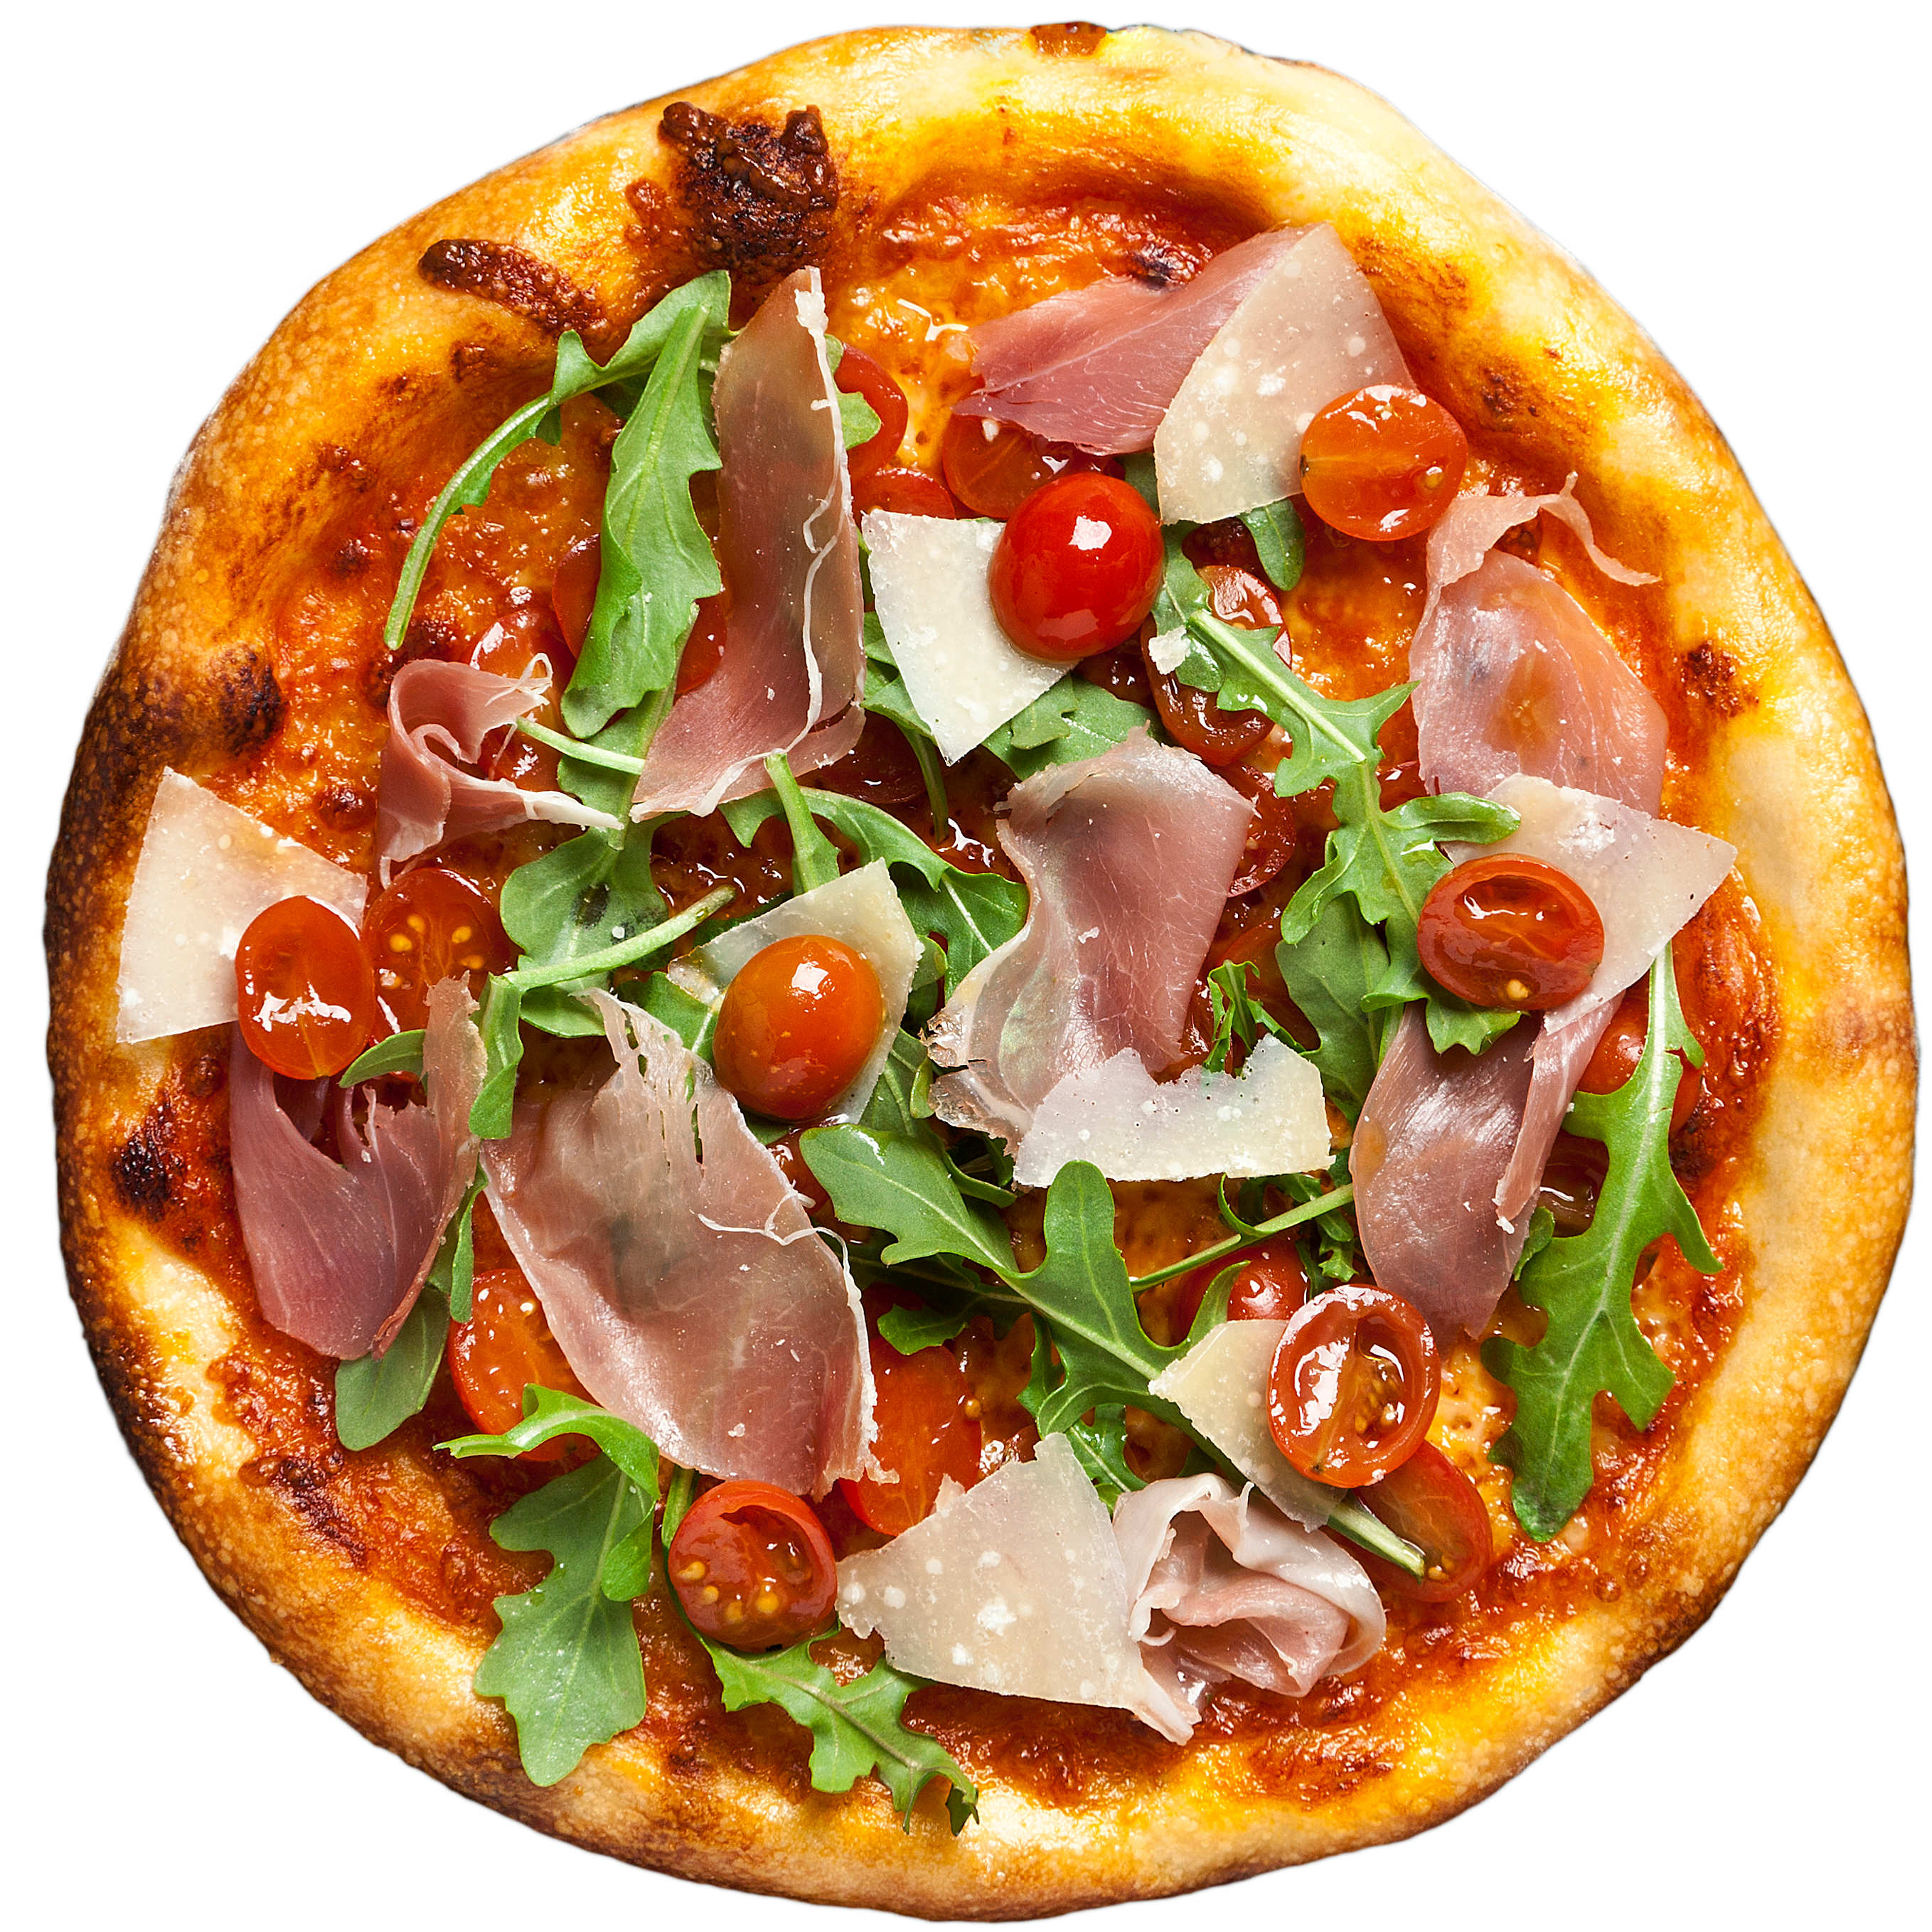
\includegraphics[width=2.5in]{img/image.png}
		\caption{Image caption.}
		\label{pic:image}
	\end{figure}

	\begin{table}[!t]
	\renewcommand{\arraystretch}{1.3}
	\caption{An Example of a Table}
	\label{table_example}
	\centering
	\begin{tabular}{|c||c|}
	\hline
	One & Two\\
	\hline
	Three & Four\\
	\hline
	\end{tabular}
	\end{table}
	
	\section{Conclusion}
	The conclusion goes here.
	
	\section*{Acknowledgment}
	The authors would like to thank...
	
	\bibliographystyle{plain}
	\bibliography{main}
\end{document}


